\chapter{Introduction}
\label{ch:intro}
%The goal of this work is to extend faceted search into an open-domain web setting. In this introduction, we first provide some background about faceted search in Section~\ref{sec:intro-paradigms} and \ref{sec:intro-fs}. Then we will provide motivations for extending faceted search to the open-domain web setting in Section~\ref{sec:intro-motivation}. Then we propose Faceted Web Search (faceted search in the open-domain web setting) and describe the fundamental issues in Facet Web Search in Section~\ref{sec:intro-fws}. After that, we highlight the contributions of the thesis in Section~\ref{sec:intro-contributions}. Lastly, we provide an outline of the thesis in Section~\ref{sec:intro-outline}.


%\section{Two Search Paradigms}
%\label{sec:intro-paradigms}
There are primarily two search paradigms in use since the very beginning of web search, navigational search and direct search. Navigational search uses a hierarchy structure (taxonomy) to enable users to browse the information space by iteratively narrowing the scope of their quest in a predetermined order, as exemplified by Yahoo! Directory\footnote{http://en.wikipedia.org/wiki/Yahoo!\_Directory} and the Open Directory Project\footnote{http://www.dmoz.org/}. Taxonomies provide a guided search interface, and support abstractions that are easily understood by users. However, the strict ordering of a taxonomy can be too rigid, especially for large and heterogeneous corpora. The rapid decline of Yahoo! Directory as a primary web search engine provides pragmatic evidence.

Direct search instead allows users to specify their own queries as input, resorts to search systems for understanding search intents behind user queries, and returns search results that could best address the search intents. This approach has been made enormously popular by web search engines, such as Google\footnote{http://www.google.com}. However, in the basic search interface, users have to formulate their queries with no or limited assistance, and no exploration capability since results are presented as a flat list with no systematic organization. Recent advances, including query suggestions and search result clustering, address part of these problems and will be reviewed in Chapter~\ref{ch:bg}.

%\section{Faceted Search}
%\label{sec:intro-fs}
A third approach that combines the two search paradigms emerged during the 1990s, namely faceted search. More specifically, faceted search enables users to navigate a multi-dimensional information space by combining direct search with narrowing choices in each dimensions, which are also called facets. For example, consider looking for a computer monitor in an e-commerce site like Amazon\footnote{http://www.amazon.com}. Users can directly search with the query \concept{computer monitor}. However, the number of computer monitors retrieved could be overwhelming. To assist users in refining and exploring the search results, the site provides refining choices in each facets. In this case, the facets are computer monitor attributes, such as \concept{brand} with the choices \{\concept{Dell}, \concept{ViewSonic}, \concept{HP}, ...\}, \concept{display technology} with the choices \{\concept{LED-Lit}, \concept{LCD}, ...\}, and \concept{condition} with the choices \{\concept{new}, \concept{used}, \concept{refurbished}\}
, 
as illustrated in Figure~\ref{fig:intro-amazon}. Then users can select some of the provided choices and combine them to refine the search results. For example, users can select the choice \concept{new} from the facet \concept{condition} to request only computer monitors in new conditions. Users can also combine the choice \concept{Dell} in the facet \concept{brand} with the choice \concept{LCD} in the facet \concept{display technology} to request only Dell computer monitors with LCD display technology.

\begin{figure}[!ht]
\centering
\includegraphics[width=0.95\columnwidth]{figure2/amazon.png}
\caption{Faceted search illustrated by an example searching ``computer monitor'' in Amazon. The search interface shown has been simplified for the convenience of illustration.}
\label{fig:intro-amazon}
\end{figure}

% Compare with direct search
Compared with direct search, faceted search provides additional search assistance for users. The facts provided in faceted search can assist users in clarifying their search intent and refining the search results, as already illustrated in the computer monitor example above. In addition, faceted search supports guided exploration over the complex information space. In the computer monitor example above, without the provided facets, users might have no clue about how to explore the large amount of returned results. By listing computer monitor attributes as facets, the site gives users an overview of the returned results, and provides them with the key factors they may need to consider when searching for a computer monitor. In other words, using facets, the site summarizes the search space succinctly, and provides exploration suggestions organized in an systematic way. This exploration capability is especially important in exploratory search tasks, or when users are not exactly clear about what they are 
looking for.

% Compare with navigational search
Compared with navigational search, faceted search is different not only in its direct search capability, but also in its navigation mechanism. Navigation in navigational search is typically based on one single taxonomy that organizes information objects in a hierarchy structure. The key property of such a taxonomy is that, for every object in the taxonomy, there is precisely one unique path to it from the taxonomy root. For example, \concept{cancer} can be classified in a taxonomy with a unique path  \concept{disease}$\rightarrow$\concept{structural disease}$\rightarrow$\concept{tumor}$\rightarrow$\concept{cancer}. However, this strict ordering of a taxonomy can be too rigid when dealing with compound information objects. For example, should \concept{treatment of cancer} be a child of \concept{treatment} or of \concept{cancer}? This strict ordering constraint limits expressibility and extensibility of taxonomy. 
%We will discuss more on this issue in Chapter~\ref{ch:bg}.

Instead, in faceted search, navigation is based on multiple independent taxonomies, called faceted taxonomies or multi-dimensional taxonomies. Each of the taxonomies organizes information objects from a different (preferably orthogonal) point of view, or equivalently in a different dimension of the multi-dimensional information space. The independent taxonomies in a faceted taxonomy can also be called \concept{facets}. However, \concept{facets} are often used to indicate the part of independent taxonomies that are shown to users, and in many cases the taxonomies are often shown as shallow trees. In the computer monitor example above, the facets show only two-level taxonomies (\eg, node \concept{Brand} with children \concept{Dell}, \concept{ViewSonic}, etc.). We will provide a more detailed explanation of facets and related concepts in Chapter~\ref{ch:bg}.
 
Combining these independent taxonomies, a faceted taxonomy offers expressive power and flexibility beyond a single taxonomy used in navigational search. Ranganathan
first proposed the idea of faceted taxonomy in library science. In \textit{Classification, Coding, and Machinery for Search}~\cite{ranganathan1950classification}, he provided an example that expresses the topic \concept{statistical study of the treatment of cancer of the soft palate by radium} based on four constituent taxonomies in a faceted taxonomy as follows.
\begin{itemize}
 \item Medicine $\rightarrow$ Digestive system $\rightarrow$ Mouth $\rightarrow$ Palate $\rightarrow$ Soft palate
\item Disease $\rightarrow$ Structural disease $\rightarrow$ Tumor $\rightarrow$ Cancer
\item Treatment $\rightarrow$ Treatment by chemical substances $\rightarrow$ Treatment by a chemical element  $\rightarrow$ Treatment by a group 2 chemical element $\rightarrow$ Treatment by radium
\item Mathematical study $\rightarrow$ Algebraical study $\rightarrow$ Statistical study
\end{itemize}
In the example, the four taxonomies (\concept{Medicine}, \concept{Disease}, \concept{Treatment} and \concept{Mathematical study}) each represents one dimension of the information space. The foci in each of the taxonomies (\concept{Soft palate}, \concept{Cancer}, \concept{Treatment by radium} and \concept{Statistical study}) are combined to express the compound topic, which is difficult in a single hierarchical taxonomy.
%pose a challenge for the hierarchical organization of single taxonomies.



In summary, faceted search combines direct search with navigation based on a faceted taxonomy, providing assistance for users in clarifying search intent and exploration over a multi-dimensional information space. It has also been used successfully for many vertical applications, such as e-commerce and digital libraries. 
%User studies demonstrate that faceted search provides more effective information-seeking support to users~\cite{sacco2009dynamic}\todo{need a more appropriate citation}. 

\section{Motivation for Faceted Web Search}
\label{sec:intro-motivation}
While the principles of faceted taxonomy are widely applicable, faceted search has not been explored much for general web search in an open-domain setting. There is lots of work studying faceted search in fixed domain such as images~\cite{cutrell2006fast}, movies~\cite{koren2008personalized}, houses~\cite{shneiderman1994dynamic}, and desktop content~\cite{cutrell2006fast}. However, there is limited work in successfully extending faceted search to the open-domain, due to the challenges of the large and heterogeneous nature of the web~\cite{teevan2008challenges}.

Nevertheless, faceted search naturally suits and holds great potential for assisting multi-faceted queries and exploratory search in the open-domain web setting. We illustrate the idea with four example queries and their facets manually created in Table~\ref{tab:facetexample}. For the first query \concept{baggage allowance}, the facet of different airlines (facet 1) can assist users to quickly compare baggage policies between different airlines. Users can also use other facets, such as flight types, flight classes and specifications to clarify this multi-faceted query. 
%For the second query, \concept{Mr Bean}, the facets succinctly summarize interesting aspects for the Mr. Bean television series, including episodes titles (facet 2), casts (facet 3) and characters (facet 4). This information could help users to learn and explore this topic. 
For the second query, \concept{Mars landing}, the facets list important information for exploring this topic, including Mars rovers (facet 1) and countries relevant to Mars landing (facet 2). Users can also combine multiple facets for search intent  clarification (e.g., select \concept{Curiosity} from facet 1 and \concept{pictures} from facet 3 to find pictures of Mars rover Curiosity). The last query shows that faceted search is not limited to short queries. The facets succinctly summarize interesting aspects for the complex query \concept{Effect of building the three gorges dam in China}, including  different types of effect (facet 1), related nature disasters (facet 2) and different regions of the river (facet 3). This information could help users to learn and explore this topic.
\begin{table}[!ht]
\centering
\caption{Examples facets for three web search queries.}
\label{tab:facetexample}
\begin{tabular}{|l|} \hline
Query 1: baggage allowance \\\hline
Facet 1: AA, Delta, Jetblue,  ... \\
Facet 2: international, domestic \\
Facet 3: first class, business class, economy class \\
Facet 4: weight, size, quantity \\\hhline{|=|}
%Query 2: Mr Bean \\\hline
%Facet 1: comics, movies, tv, books \\
%Facet 2: The Curse of Mr Bean, Mr Bean Goes to Town, ...\\
%Facet 3: Rowan Atkinson, Richard Wilson, Jean Rochefort,  ...\\ 
%Facet 4: Mr Bean, Irma gobb, Rupert, Hubert, ...\\\hhline{|=|}
Query 2: Mars landing \\\hline
Facet 1: Curiosity, Opportunity, Spirit \\
Facet 2: USA, UK, Soviet Union \\
Facet 3: video, pictures, news \\\hline
Query 3: Effect of building the three gorges dam in China \\\hline
Facet 1: environmental, social, economic \\
Facet 2: landslides, soil erosion, earthquake\\
Facet 3: lower, middle, upper \\\hline
\end{tabular}
\end{table}

Faceted search when extended to the open-domain web setting can have several advantages over other related techniques developed for faceted queries or exploratory search. Search result diversification has been studied as a method of tackling ambiguous or multi-faceted queries while a ranked list of documents remains the primary output feature of web search engine today~\cite{agrawal2009diversifying,clarke2008novelty,santos2010exploiting,sakai2011evaluating,dang2013term}.
The purpose is to diversify the ranked list to account for different search intents or query subtopics. However, the query subtopics are hidden from the user, leaving him or her to guess at how the results are organized. Faceted search addresses this problem by explicitly presenting different facets for the search topic.

Search results clustering or organization is a technique that tries to organize search results by grouping them into clusters~\cite{carpineto2009survey} or organizing them in a single hierarchical taxonomy~\cite{lawrie2001finding,lawrie2003generating, nevill1999lexically}, very much like in navigational search. This offers a complementary view to the flat ranked list of search results. However, single taxonomies or fixed clusters, as mentioned before, impose strict taxonomic ordering for the search results. Instead, faceted search allows users to explore the search space from multiple facets, offering flexibility beyond search results clustering or organization.

Query suggestion~\cite{baeza2004query, cao2008context} is a technique that generates alternative queries for users to helps them explore or express their information need. This technique is now widely used in commerce web search engine. However, the suggested queries are often provided in a flat list with no systematic organization and no capability of combining multiple suggestions. Instead, ``suggestions'' in faceted search are organized systematically into facets, which makes it conceptually easier to browse and select.

\section{Faceted Web Search}
\label{sec:intro-fws}
In this thesis, we extend faceted search into the open-domain web setting, which we call Faceted Web Search (FWS). Similar to conventional faceted search, a FWS system will provide facets when a user issues a web search query. The user can then select some choices from the facets, which will be used by the FWS system to adjust the search results to better address the user's information need.

We illustrate the idea of FWS in Figure~\ref{fig:fws-example}, supposing a user is preparing for an international flight and wants to find baggage allowance information. When the user searches ``baggage allowance'' in an FWS system (step 1 in the figure), in addition to the search result list (step 2), the system will provide a list of facets (step 3), such as a facet for different airlines, \{\textit{Delta}, \textit{JetBlue}, \textit{AA}, ...\}, a facet for different flight types, \{\textit{domestic}, \textit{international}\}, and a facet for different classes, \{\textit{first}, \textit{business}, \textit{economy}\}. When the user selects choices such as ``Delta'', ``international'' and ``economy'' in these facets (step 4), the system can ideally help to bring web documents that provide 
baggage allowance information for the economy class of Delta international flights to the top of the search results (step 5).
\begin{figure}[!ht]
\centering
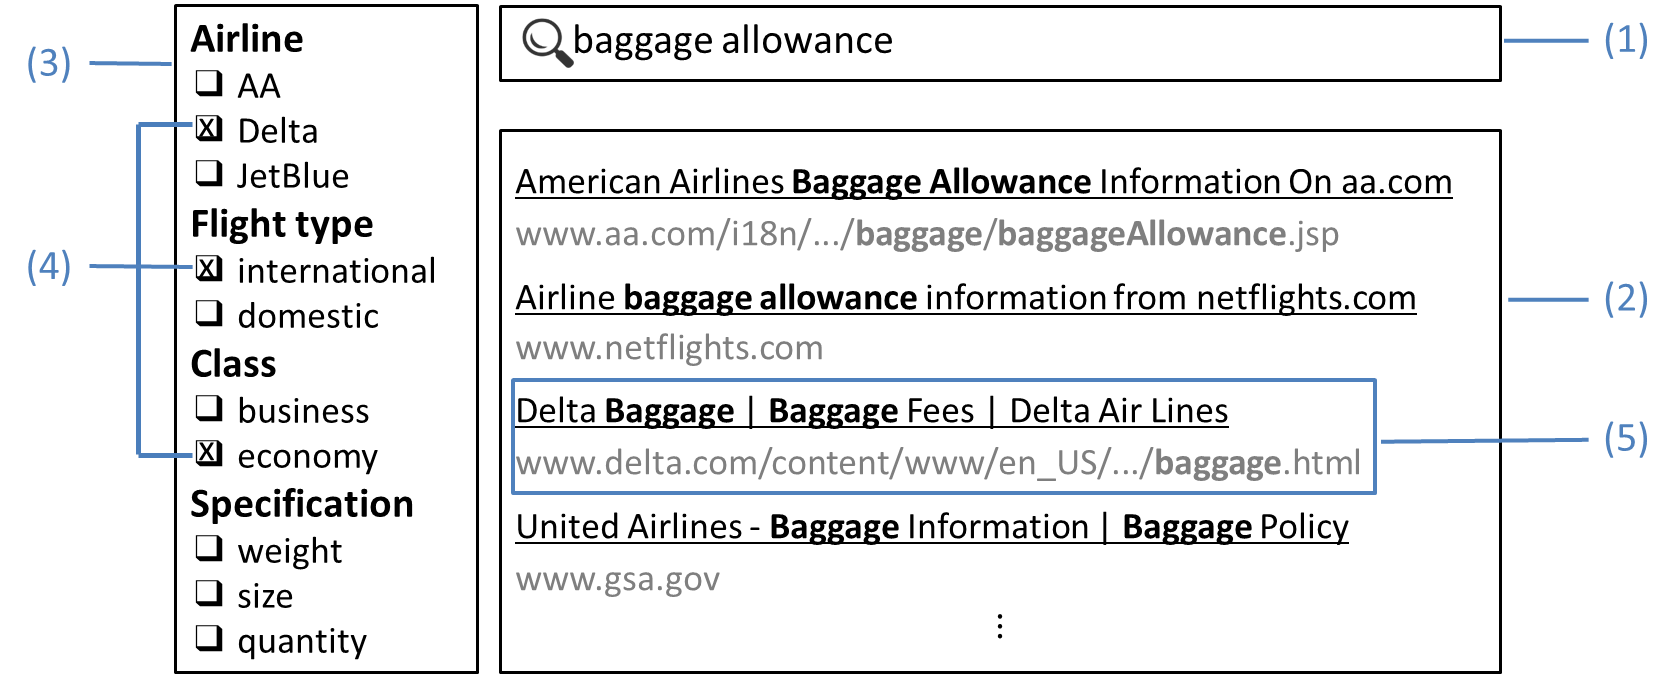
\includegraphics[width=0.97\columnwidth]{figure/fws-example.png}
%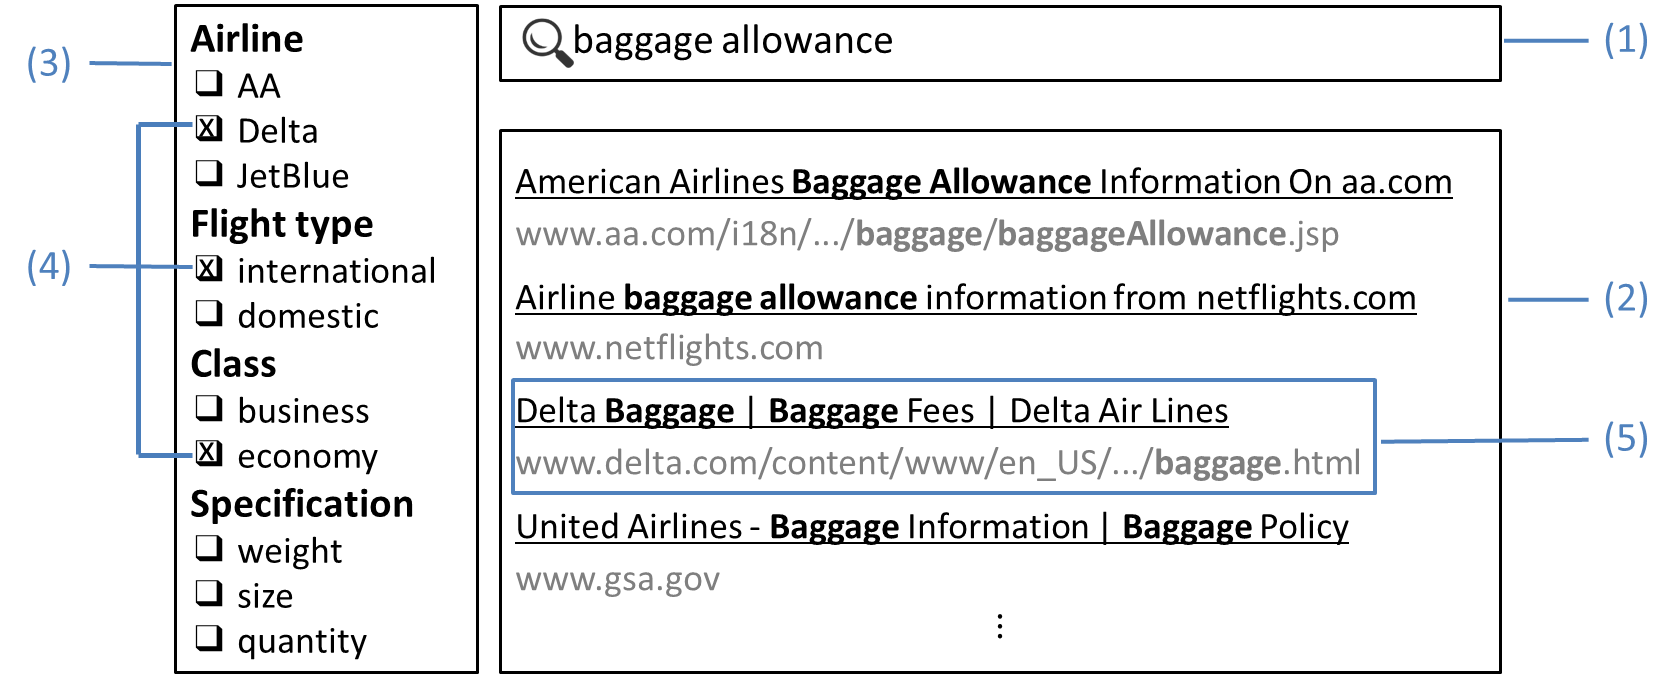
\includegraphics[scale=0.45]{figure/fws-example.png}
\caption{An example of Faceted Web Search: (1) the user issues a query; (2) the system returns search results; (3) the system provides facets for the query; (4) the user selects terms in the facets; (5) the system re-ranks this relevant document to the top according to the selected terms.}
\label{fig:fws-example}
\end{figure}


This thesis address three fundamental issues of Faceted Web Search, including facet generation, facet feedback, and evaluation, as described further as follows.

\subsection{Facet Generation}
Facet generation is to identify facets for navigation (corresponding to step 3 in Figure~\ref{fig:fws-example}). In conventional faceted search, facets are generated in advance for an entire corpus~\cite{stoica2007automating,dakka2008automatic} either manually or semi-automatically, and then recommended for particular queries in most of the previous work~\cite{teevan2008challenges}. However, this approach is difficult to extend to the entire web due to the web's large and heterogeneous nature. We instead propose a query-dependent approach, which extracts facets for a query from its search results, providing a promising direction for solving the problem. 

We call the extracted items ``query facets'', defined as a set of coordinate terms (\eg, \{\concept{AA}, \concept{Delta}, \concept{JetBlue},...\}) that explicitly represent one aspect (\eg, \concept{airlines}) of the query (\eg, \concept{baggage allowance}). The coordinate terms share a semantic relationship by being subsumed by a more general hypernym (\eg, \concept{AA}, \concept{Delt}, \concept{JetBlue} are subsumed by \concept{airlines}). More examples for query facets are shown in Table~\ref{tab:facetexample}. Note that our work dose not generate the hypernym or label (\eg, \concept{airlines}) for the coordinate terms. This definition of query facets corresponds to one-level taxonomies in faceted taxonomy, in which only information objects that belong to a same parent node are shown as a facet (see the definition in Section~\ref{sec:bg-fws}). We leave generating facets as two- or more level taxonomies as future work.

Because it is an automatic task, facet generation in FWS can be imperfect. The system can make mistakes in both precision and recall for generating facets. As in many precision-oriented information retrieval tasks, we believe users are likely to care more about ``facet precision'' than ``facet recall''. That is, users may care more about the correctness of presented facets (\eg, are the terms in the airline facet indeed about airlines, and are the airline terms grouped together in a same facet) than the completeness of facets (\eg, are all possible facets for that query presented, and are all possible airline terms included the results?). In other words, mistakes of presenting wrong terms in a facet, or grouping terms incorrectly are more severe than omitting some facets or terms in facets. Thus, we also study how to improve facet generation performance under precision-oriented scenarios, in order to make the technique more practical.

\subsection{Facet Feedback}
Facet feedback is to use selections on the facets to adjust (\eg, filter or re-rank) the search results (corresponds to step 5 in Figure~\ref{fig:fws-example}). In conventional faceted search, facet feedback is straightforward: as all information objects have been classified in the faceted taxonomy, when users make their selections on the facets, the search results can be easily filtered by requiring each objects belong to the restricted taxonomies according to the selection.

However, in FWS there is no explicit classification of webpages into the generated facets. One solution is Boolean filtering, which filters search results by the requiring selected terms to appear. However, it turns out to be too strict when extended to the open-domain setting. Boolean filtering is based on two assumptions~\cite{zhang2010interactive}: (1) users are clear about what they are looking for, and thus are able to select proper terms to restrict the results; and (2) matching between a term and a document is accurate and complete. In FWS, that means a document that contains the selected term should be relevant to the term, and all documents relevant to that selected term should contain the term. Neither of the two assumptions are likely to hold reliably in FWS. Thus, we also investigate soft ranking models that expand original queries with user selection on the facets.
  

\subsection{Evaluation}
Evaluation for conventional faceted search mostly focuses on its user interface~\cite{burke1996knowledge,english2002hierarchical,hearst2006design,hearst2008uis,kules2009exploratory}. For FWS, there can be two types of evaluation according to the different focuses, namely intrinsic and extrinsic evaluation. Intrinsic evaluation only considers facet generation (i.e., the quality of generated facets).  Extrinsic evaluation instead evaluates the effectiveness of the entire FWS system, combining both the facet generation and facet feedback components. We study both of them.

Most of the previous evaluations for faceted search are based on user studies~\cite{dash2008dynamic,li2010facetedpedia,stoica2007automating}. However, user studies are often very expensive and more importantly difficult to extend for evaluating new systems. We instead design evaluation methods with higher reusability for both intrinsic and extrinsic evaluation.

In the following, we highlight the contributions of this thesis.
\section{Contributions}
\label{sec:intro-contributions}
\begin{itemize}
 \item Faceted Web Search. We define Faceted Web Search, which extends faceted search into an open-domain web setting. We design a framework for an FWS system, which contains the facet generation and facet feedback components. We show that using this faceted search interface can significantly improve the original ranking if allowed sufficient time for user feedback: 18.0\% in NDCG@10 if we allow users to examine 50 terms in facets, and 7.4\% in NDCG@10 if we allow time for examining 10 terms. \todo{interactive}

 \item Query facet extraction. To cope with the large and heterogeneous nature of the web in facet generation, we develop a query-dependent approach, which generates facets for a query instead of the entire corpus. This query facet generation approach extracts facets from the top search results for the issued query. This not only makes the generation problem easier, but also addresses the facet recommendation problem at the same time. For query facet extraction, we develop a supervised approach based on a graphical model to recognize facets from the noisy candidates found. The graphical model learns how likely a candidate term is to be a facet term as well as how likely two terms are to be grouped together in a query facet, and captures the dependencies between the two factors. We propose two algorithms (\QFI and \QFJ) for approximate inference on the graphical model since exact inference is intractable. Compared with other existing methods, our models can easily incorporate a rich set of features, and learn for available labeled data.

\item Intrinsic evaluation. We evaluate the quality of generated facets by comparing them with human-created ones. This can be measured from three aspects -- precision and recall of extracted terms for facets, and the clustering quality of these facet terms. We design \PRF, a measure to combine three evaluation factors together using weighted harmonic mean. This metric has the flexibility to adjust emphasis between the three factors for different applications. We also describe how to collect human annotations for query facets by a pooling method. Experimental results based on this intrinsic evaluation show that our supervised methods (\QFI and \QFJ), can take advantage of a richer set of features and outperform other unsupervised methods, such as pLSA, LDA, and a variant of quality threshold clustering model~\cite{dou2011finding}. \todo{pooling for annotation}

\item Precision-oriented query facet extraction. We improve query facet extraction performance under precision-oriented scenarios from two perspectives. First, we find that the likelihood objective used in the query facet extraction model can be loosely related to the performance measure in the precision-oriented scenario. Therefore, we directly optimize the performance measure instead of likelihood during training using a empirical utility maximization approach. However, exact optimization on the performance measure is difficult due to the non-continuous and non-differentiable nature of information retrieval measures. We address this problem by approximating the performance measure using its expectation. We show that this empirical utility maximization approach significantly improves models under precision-oriented scenarios, suggesting that utility is a better learning objective than likelihood, and that our expectation-based approximation is effective.  


\item Second, we improve extraction performance by a selective method that shows facets for good performing queries and avoids doing so for poor performing ones. We find that extraction performance varies for different queries -- some queries are naturally more difficult than others for extracting query facets. In the precision-oriented scenario, it may be more desirable to avoid showing facets for those poor performing queries and leave the users with a clean keyword-search interface. A key problem, however, is how to predict the extraction performance. To solve this problem, we develop a simple and effective score based on the expectation of the performance measure. We find the score has a strong correlation with the performance measure, and when used in the selective method, it can significantly improve the average performance with fair coverage over the whole query set.

 
\item Facet feedback. We find that Boolean filtering models are too strict for FWS, and propose soft ranking models that expand original queries with user selected terms in facets for re-ranking. We show that the proposed soft ranking models are more effective than Boolean filtering models, which are widely used in conventional faceted search.
 
\item Extrinsic evaluation. We develop an extrinsic evaluation method that evaluates FWS systems by their utility in assisting search clarification. This evaluation considers both gain in ranking improvement and cost in time for users to give feedback. Instead of performing user studies, we simulate the user feedback process, so that we can easily extend the evaluation for new models or systems. The simulation is based on a simple user model of the feedback process and limited human annotations.

\item Building a reusable test collection. We describe a way of building reusable test collections for the intrinsic and extrinsic evaluation. We make our collected data set publicly available. The data set consists of annotated facets for 196 TREC Web Track queries from 2009 to 2012, and simulated user feedback for 678 corresponding query subtopics.

%\item A demonstration system for Faceted Web Search. We develop a demonstration system
%%\footnote{It is currently online in http://brooloo.cs.umass.edu/}
%for Faceted Web Search. The demonstration system shows extracted query facets for a given query online. The system now supports querying over the entire web using Bing Search API\footnote{https://datamarket.azure.com/dataset/bing/search}, and ClueWeb09 corpus\footnote{http://lemurproject.org/clueweb09} based on Galago Search Engine\footnote{http://www.lemurproject.org/galago.php}.
\end{itemize}

\section{Outline}
The remainder of this thesis is organized as follows. 
In Chapter~\ref{ch:bg}, we provide background information related to this thesis. In Chapter~\ref{ch:facet}, we present our query facet extraction approach. 
In Chapter~\ref{ch:intrinsiceval}, we present our intrinsic evaluation that evaluates generated facets by comparing them with human-created ones.
In Chapter~\ref{ch:precision}, we investigate query facet extraction models under precision-oriented scenarios, and improve our models in such scenarios.
In Chapter~\ref{ch:feedback}, we investigate both Boolean filtering and soft ranking models for facet feedback.
In Chapter~\ref{ch:extrinsiceval}, we develop our extrinsic evaluation method that evaluates entire Faceted Web Search systems in terms of their utility in assisting search in an interactive search task.
Lastly, in Chapter~\ref{ch:conclusions}, we summarize the contributions made in this thesis and discuss potential future directions for more research in this area.




